\documentclass[10pt,a4paper,twocolumn]{article}
% The following LaTeX packages must be installed on your machine: amsmath, authblk, bm, booktabs, caption, dcolumn, fancyhdr, geometry, graphicx, hyperref, latexsym, natbib
\input{151.dat}
\usepackage{gensymb}
\usepackage{amsthm}
\usepackage{float}
\usepackage{siunitx}
\usepackage{amssymb}
\usepackage{float}
\usepackage{enumerate}
\usepackage{listings}
\usepackage{mathtools}
\PassOptionsToPackage{hyphens}{url}\usepackage{hyperref}
\usepackage[none]{hyphenat}
\usepackage{physics}
\usepackage{chngcntr}
\counterwithin*{equation}{section}
\newcommand\ddfrac[2]{\frac{\displaystyle #1}{\displaystyle #2}}
%\renewcommand{\familydefault}{\sfdefault}


\begin{document}

\begin{titlepage}
\begin{center}
\vspace*{\fill}

\normalsize{Physics 151 \\
Crib Sheet \\
2nd semester, A.Y. 2018-19} \\

\qquad
\qquad

\normalsize{Kenneth V. Domingo \\
2015-03116 \\
28}

\vspace*{\fill}
\end{center}
\end{titlepage}

\tableofcontents

\clearpage

\setcounter{page}{1}

\section[P09 PS02 2.8 Work in a cyclic process]{P09 PS02 2.8}
Consider the cyclic process as described in Example 2.1.

\begin{figure}[htb]
	\centering
	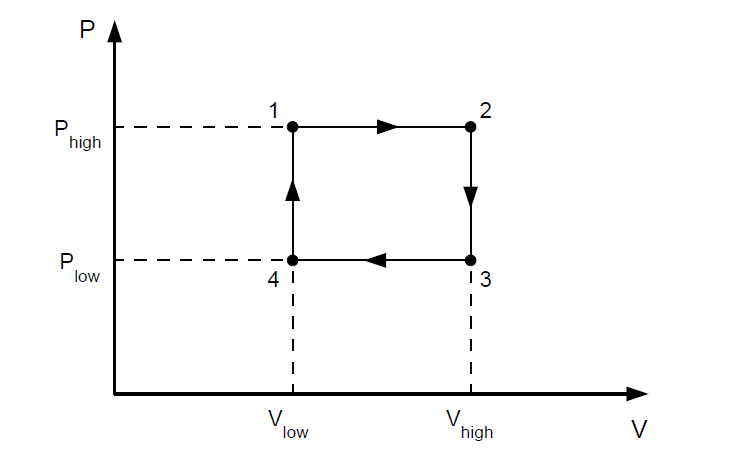
\includegraphics[width=0.75\linewidth]{work.png}
	\caption{Cyclic process for this problem.}
	\label{fig:2.8-cycle}
\end{figure}

\begin{enumerate}[(a)]
	\item Because the system was returned to its original pressure and volume, why is the net amount of work done on the system not zero?
	
	The net work done on the system is non-zero since it depends on the initial, intermediate, and final macrostates (i.e. the path).
	
	\item What would be the work done on the gas if the gas were taken from $1 \rightarrow 2 \rightarrow 3$ and then back to 1 along the diagonal path connecting 3 and 1?

\begin{align}
	W_{1 \rightarrow 2} &= P_{high}\qty(V_{high} - V_{low}) \\
	W_{2 \rightarrow 3} &= \qty(P_{low} - P_{high})V_{high} \\
	W_{3 \rightarrow 1} &= \sqrt{P_{high}^2\qty(V_{high} - V_{low})^2 + \qty(P_{low} - P_{high})^2 V_{high}^2} \\
	W_{net} &= W_{1 \rightarrow 2} + W_{2 \rightarrow 3} + W_{3 \rightarrow 1}
\end{align}

\end{enumerate}


\section{P10 PS02 2.13}
In Example 2.1 we showed that the net work done on the gas in the cyclic process shown in Figure \ref{fig:2.8-cycle} is nonzero. Assume that the gas is ideal with N particles and calculate the energy transfer by heating in each step of the process. Then explain why the net work done on the gas is negative and show that the net change of the internal energy is zero.

From Example 2.1, the net work done on a gas in a cyclic process was determined to be nonzero, with a value of

\begin{equation}\label{oldanswer}
	W_{net} = -\left( P_{high} - P_{low} \right) \left( V_{high} - V_{low} \right)
\end{equation}

Assuming an ideal gas with $N$ particles, the energy transfer due to heating for each step in the process is as follows:

\begin{align}
	Q_{1 \rightarrow 2} = -Q_{3 \rightarrow 4} & = \int_{T_1}^{T_2} c_P \textrm{ d}T \\
	& = \nu c_P \int_{T_1}^{T_2} \textrm{ d}T \\
	& = \nu c_P \left( T_2 - T_1 \right) \\
	& = \nu c_P \Delta T \label{eq:isobaric} \\
	Q_{2 \rightarrow 3} = -Q_{4 \rightarrow 1} & = \int_{T_1}^{T_2} c_V \textrm{ d}T \\
	& = \nu c_V \int_{T_1}^{T_2} \textrm{ d}T \\
	& = \nu c_V \left( T_2 - T_1 \right) \\
	& = \nu c_V \Delta T \label{eq:isochoric}
\end{align}

Recalling the ideal gas equation,

\begin{eqnarray}
	PV = \nu RT \label{eq:idealgas} \\
	T = \frac{PV}{\nu R} \label{eq:idealtemp}
\end{eqnarray}

The net energy transfer due to heating is

\begin{equation}\label{eq:totalwork}
	W_{net} = Q_{1 \rightarrow 2} + Q_{2 \rightarrow 3} + Q_{3 \rightarrow 4} + Q_{4 \rightarrow 1}
\end{equation}

Plugging \eqref{eq:idealtemp} into each of the equations in \eqref{eq:isobaric} and \eqref{eq:isochoric}, we have

\begin{align}
	Q_{1 \rightarrow 2} & = \nu c_P P_{high} \frac{V_{high} - V_{low}}{\nu R} \label{eq:Q12plug} \\
	Q_{2 \rightarrow 3} & = \nu c_V V_{high} \frac{P_{low} - P_{high}}{\nu R} \label{eq:Q23plug} \\
	Q_{3 \rightarrow 4} & = \nu c_P P_{low} \frac{V_{low} - V_{high}}{\nu R} \label{eq:Q34plug} \\
	Q_{4 \rightarrow 1} & = \nu c_V V_{low} \frac{P_{high} - P_{low}}{\nu R} \label{eq:Q41plug}
\end{align}

Simplifying equations \eqref{eq:Q12plug} through \eqref{eq:Q41plug} and summing them as in \eqref{eq:totalwork}, we have

\begin{align}
	Q_{net} & = c_P P_{high} \frac{V_{high} - V_{low}}{R} \nonumber \\
	& - c_V V_{high} \frac{P_{high} - P_{low}}{R} \nonumber \\
	& - c_P P_{low} \frac{V_{high} - V_{low}}{R} \nonumber \\
	& + c_V V_{low} \frac{P_{high} - P_{low}}{R}
\end{align}
\begin{align}
	Q_{net} & = \frac{c_P}{R} \left( P_{high} - P_{low} \right) \left( V_{high} - V_{low} \right) \nonumber \\
	& -\frac{c_V}{R} \left( P_{high} - P_{low} \right) \left( V_{high} - V_{low} \right) \label{eq:Wnetplug}
\end{align}

Recall that for an ideal gas,

\begin{eqnarray}
	c_P = \frac{5}{2} R \label{eq:idealcp} \\
	c_V = \frac{3}{2} R \label{eq:idealcv}
\end{eqnarray}

Plugging these into \eqref{eq:Wnetplug},

\begin{align}
	Q_{net} & = \frac{5}{2} R \frac{1}{R} \left( P_{high} - P_{low} \right) \left( V_{high} - V_{low} \right) \nonumber \\
	& -\frac{3}{2} R \frac{1}{R} \left( P_{high} - P_{low} \right) \left( V_{high} - V_{low} \right) \label{eq:Wnetideal}
\end{align}

Which gives us the expected relation of $Q_{net} = -W_{net}$ (negative because in a cyclic process, there is no change in internal energy; the work done is equal to the heat added):

\begin{equation}\label{eq:answer}
	Q_{net} = \left( P_{high} - P_{low} \right) \left( V_{high} - V_{low} \right)
\end{equation}

From the first thermodynamic law,

\begin{equation}\label{eq:1stlaw}
	\Delta E = Q + W
\end{equation}

Plugging equations \eqref{oldanswer} and \eqref{eq:answer} into this, we have

\begin{equation}\label{eq:energychange}
	\Delta E = 0
\end{equation}

\section{P11 PS03 2.15}
Use (2.44) and the ideal gas pressure equation of state in (2.8) to show that in a quasistatic adiabatic processes $P$ and $V$ are related as

\begin{equation}
	PV^\gamma = \textrm{constant}
\end{equation}

Also show that $T$ and $P$ are related as

\begin{equation}
	TP^{(1-\gamma)/\gamma} = \textrm{constant}
\end{equation}

The given equations are:

\begin{eqnarray}
	TV^{\gamma-1} = C \label{eq:given1} \\
	PV = \nu RT \label{eq:idealgaslaw}
\end{eqnarray}

Isolating $T$ in \eqref{eq:idealgaslaw},

\begin{equation}
	T = \frac{PV}{\nu R} \label{eq:idealgastemp}
\end{equation}

Plugging this into \eqref{eq:given1},

\begin{align}
	\frac{PV}{\nu R} V^{\gamma - 1} = C \nonumber \\
	PV^{\gamma} = C\nu R = C
\end{align}

Therefore,

\begin{equation}\label{eq:answer1}
\boxed{	PV^\gamma = \textrm{constant}}
\end{equation}

Similarly, isolating $V$ from \eqref{eq:idealgaslaw},

\begin{equation}\label{eq:idealgasvol}
	V = \frac{\nu RT}{P}
\end{equation}

Plugging this into \eqref{eq:answer1},

\begin{align}
	P\left( \frac{\nu RT}{P} \right)^\gamma & = C \nonumber \\
	\left( \nu RT \right)^\gamma P^{1-\gamma} & = C \nonumber \\
	T^\gamma P^{1-\gamma} & = \frac{C}{\left( \nu R \right)^\gamma} \nonumber \\
	T^\gamma P^{1-\gamma} & = D
\end{align}

Raising both sides to $1/\gamma$,

\begin{eqnarray}
	\left( T^\gamma P^{1-\gamma} \right)^{\frac{1}{\gamma}} = D^{\frac{1}{\gamma}} \nonumber \\
\boxed{	TP^{(1 - \gamma)/\gamma} = \textrm{constant}} \label{eq:answer2}
\end{eqnarray}

\section[P12 PS03 2.17 Compression of air]{P12 PS03 2.17}
\begin{enumerate}[(a)]

\item Air initially at $20^\circ$C is compressed by a factor of 15. Assuming adiabatic conditions, $V_i/15 = V_f$, $T_i = 293$K, and $\gamma = 1.4$,

\begin{eqnarray}
	TV^{\gamma -1} = C \label{eq:adiabatic} \\
	T_i V_i^{\gamma-1} = T_f V_f^{\gamma - 1} \nonumber \\
	293 V_i^{0.4} = T_f \left( \frac{V_i}{15} \right)^{0.4} \nonumber \\
	293 = T_f \left(\frac{1}{15}\right)^{0.4} \nonumber \\
	T_f = 293 \left( \frac{1}{15} \right)^{-0.4} \nonumber \\
	\boxed{T_f = 866\textrm{ K}} \label{eq:answer1}
\end{eqnarray}

Assuming air behaves like an ideal gas,

\begin{eqnarray}
	\frac{P_i V_i}{T_i} = \frac{P_f V_f}{T_f} \\
	\frac{P_i}{293}\frac{V_f}{15} = \frac{P_f V_f}{866} \nonumber \\
	\frac{P_i}{(293)(15)} = \frac{P_f}{866} \nonumber \\
	\boxed{P_i \approx 5 P_f} \label{eq:answer2}
\end{eqnarray}

	\item If the compression is isothermal,

\begin{eqnarray}
	P_i V_i = P_f V_f \\
	\boxed{P_i = 15 P_f} \label{eq:answer3}
\end{eqnarray}

	\item The pressure increases more with adiabatic compression.

\end{enumerate}

\section[P13 PS03 2.18 Work done in a quasistatic adiabatic process]{P13 PS03 2.18}

\begin{enumerate}[(a)]

\item Use the result that we derived in (2.53) to obtain the alternative form (2.54).

From the given equations,

\begin{eqnarray}
	W = C_V \left( T_2 - T_1 \right) \label{eq:workvol} \\
	PV = \nu RT \label{eq:idealgas} \\
	C_V = \frac{3}{2} \nu k_B \label{eq:volenergy}
\end{eqnarray}

Plugin \eqref{eq:idealgas} and \eqref{eq:volenergy} into \eqref{eq:workvol}:

\begin{align}
	W & = \frac{3}{2} \nu k_B \left( \frac{P_2 V_2}{\nu k_B} - \frac{P_1 V_1}{\nu k_B} \right) \nonumber \\
	& = \frac{3}{2} \left( P_2 V_2 - P_1 V_1 \right)
\end{align}

Since $\gamma = \frac{5}{3}$ for monatomic ideal gas,

\begin{align}
	W & = \frac{\left( P_2 V_2 - P_1 V_1 \right)}{\frac{2}{3}} \nonumber \\
	& = \frac{\left( P_2 V_2 - P_1 V_1 \right)}{\frac{5}{3} - \frac{3}{3}} \nonumber \\
	\Aboxed{ W & = \frac{\left( P_2 V_2 - P_1 V_1 \right)}{\gamma - 1}} \label{eq:answer1}
\end{align}

\item Show that another way to derive (2.54) is to use the relations (2.14) and (2.46).

From the given equations,

\begin{eqnarray}
	PV^\gamma = C \label{eq:constant} \\
	W = -\int_{V_1}^{V_2} P(T,V) \dd{V} \label{eq:workint}
\end{eqnarray}

Isolate $P$ from \eqref{eq:constant} and plug into \eqref{eq:workint}:

\begin{align}
	W &= -\int_{V_1}^{V_2} C V^{-\gamma} \dd{V} \nonumber \\
	& = -C \frac{V^{1 - \gamma}}{1 - \gamma} \bigg|_{V_1}^{V_2} \nonumber \\
	& = \frac{1}{\gamma - 1}\left( CV_2^{1-\gamma} - CV_1^{1-\gamma} \right) \nonumber \\
	& = \frac{1}{\gamma - 1}\left( CV_2^{-\gamma}V_2 - CV_1^{-\gamma}V_1 \right)
\end{align}

From \eqref{eq:constant},

\begin{equation}
	P = CV^{-\gamma}
\end{equation}

Therefore,

\begin{equation}\label{eq:answer2}
\boxed{	W = \frac{1}{\gamma - 1} \left( P_2 V_2 - P_1 V_1 \right) }
\end{equation}

\end{enumerate}

\section[P14 PS03 2.20 Heat pump]{P14 PS03 2.20}
A heat pump works on the same principle as a refrigerator, but the goal is to heat a room by cooling its cooler surroundings. For example, we could heat a building by cooling a nearby body of water. If we extract energy $Q_{cold}$ from the surroundings at $T_{cold}$, do work $W$, and deliver $Q_{hot}$ to the room at $T_{hot}$, the coefficient of performance is given by

\begin{equation}
	\textrm{COP} = \frac{\textrm{what you get}}{\textrm{what you pay for}} = \frac{Q_{hot}}{W}
\end{equation}

What is the maximum value of COP for a heat pump in terms of $T_{cold}$ and $T_{hot}$? What is the COP when the outside temperature is 0$^\circ$C and the interior temperature is 23$^\circ$C? Is it more effective to operate a heat pump during the winters in New England where the winters are cold or in the Pacific Northwest where the winters are relatively mild? (It is too bad that the maximum efficiency of a heat pump occurs when it is needed least.)

Since we want to heat a room surrounded by a cooler environment, the work done is positive:

\begin{align}
	\textrm{COP} &= \frac{Q_{hot}}{Q_{hot} - Q_{cold}} \\
	&= \frac{N k_B T_{hot} \ln{\left( \frac{V_f}{V_i} \right)}}{Nk_B T_{hot}\ln{\left( \frac{V_f}{V_i} \right)} - Nk_B T_{cold} \ln{\left( \frac{V_f}{V_i} \right)}} \nonumber  \\
	\Aboxed{\textrm{COP} &= \frac{T_{hot}}{T_{hot} - T_{cold}}} \label{eq:answer1}
\end{align}

Plugging the given conditions $T_{hot} = 296$K and $T_{cold} = 273$K into \eqref{eq:answer1},

\begin{align}
	\textrm{COP} &= \frac{296}{296-273} \nonumber \\
	\Aboxed{\textrm{COP} &= 12.9} \label{eq:answer2}
\end{align}

The denominator is larger for large temperature differences. The heater is more efficient in regions with mild winters.

\section[P15 PS03 2.21 Water in contact with two heat baths in succession]{P15 PS03 2.21}
The temperature of 1 kg of water at 0$^\circ$C is increased to 50$^\circ$C by first bringing it into contact
with a heat bath at 25$^\circ$C and then with a heat bath at 50$^\circ$C. What is the change in entropy of the entire system? How does this change in entropy compare with the change that was found in Example 2.15?

For the first bath,

\begin{align}\label{eq:entropy1}
	\Delta S_{11} &= C\ln{\left( \frac{T_b}{T_a} \right)} \\
	&= 4184\ln{\left( \frac{298}{273} \right)} \nonumber \\
	&= 366.6 \textrm{ J/K}
\end{align}

The energy transfer is

\begin{align}
	Q &= C \left( T_b - T_a \right) \\
	&= 4184(25) \nonumber \\
	&= 104 600 \textrm{ J}
\end{align}

So the entropy of the first bath is

\begin{align}
	\Delta S_{12} &= -\frac{Q}{T_b} \\
	&= -\frac{104 600}{298} \nonumber \\
	&= -351 \textrm{ J/K}
\end{align}

The total entropy change for the first bath is

\begin{align}
	\Delta S_1 &= 366.6 - 351 \\
	&= 15.6 \textrm{ J/K}
\end{align}

Similarly, for the second bath,

\begin{align}
	\Delta S_{21} &= 4184\ln{\left( \frac{323}{298} \right)} \\
	&= 337.1 \textrm{ J/K} \\
	\Delta S_{22} &= -\frac{Q}{T_b} \\
	&= -\frac{104 600}{323} \\
	&= -323.8 \textrm{ J/K} \\
	\Delta S_2 &= 337.1 - 323.8 \\
	&= 13.3 \textrm{ J/K}
\end{align}

The total entropy change for both processes is then

\begin{align}
	\Delta S &= 15.6 + 13.3 \\
\Aboxed{\Delta S&= 28.9 \textrm{ J/K}} \label{eq:answer1}
\end{align}


The value obtained is less than that of the water directly placed in contact with the $50^\circ$ bath.

\section[P16 PS04 2.23 More work]{P16 PS04 2.23}
\begin{enumerate}[(a)]

\item Show that the work performed by the heat engine in Example 2.19 is given by

\begin{equation}
	W = C_A \left( T_A - T \right) + C_B \left( T_B - T \right) \label{eq:prove}
\end{equation}

where $C_A$ and $C_B$ are constants and $T$ is given by (2.109) if the process is reversible. (Recall that our convention is to consider the work done on a system, except when we are discussing heat engines.)

Given

\begin{equation}\label{eq:giventemp}
	T = T_A^{\frac{C_A}{C_A + C_B}} T_B^{\frac{C_B}{C_A + C_B}}
\end{equation}

The work done by an engine on bath A for the entire process is

\begin{equation}\label{eq:workengine}
	W = -P\dd{V}
\end{equation}

From the ideal gas law,

\begin{align}
	PV = NkT \\
	\dd(PV) = \dd(NkT) \\
	P\dd{V} = Nk \dd{T} \label{eq:idealgas}
\end{align}

the temperature of bath A, from $T_A$, approaches the equilibrium temperature $T$. Express $\dd{V}$ as

\begin{equation}
	\dd{V} = \frac{Nk_B \dd{T}}{P}
\end{equation}

Plugging this into \eqref{eq:workengine},

\begin{align}
	W & = -P \frac{Nk_B\dd{T}}{P} \nonumber \\
	& = -Nk_B\dd{T} \nonumber \\
	& = -Nk_B \left( T - T_A \right) \nonumber \\
	& = Nk_B \left( T_A - T \right)
\end{align}

Define $C_A = N_A k_B$ as a constant inherent to bath A. The work done on bath A is

\begin{equation}
	W_A = C_A \left( T_A - T \right)
\end{equation}

Since the engine also does work on bath B, we can similarly define a constant inherent to bath B as $C_B = N_B k_B$. Consequently, 

\begin{equation}
	W_B = C_B \left( T_B - T \right)
\end{equation}

Thus, the total work done by the engine is

\begin{eqnarray}
	W = W_A + W_B \\
	\Aboxed{ W = C_A \left( T_A - T \right) + C_B \left( T_B - T \right) } \label{eq:answer-a}
\end{eqnarray}

\item Suppose that $C_A = C_B = C$ (a constant independent of $T$) in (2.93) and (2.109). Compare the form of the expressions for the final temperature.

\eqref{eq:giventemp} becomes,

\begin{align}
	T &= T_A^{\frac{C}{2C}} T_B^{\frac{C}{2C}} \nonumber \\
	& = T_A^\frac{1}{2} T_B^{\frac{1}{2}} \nonumber \\
	\Aboxed{ T &= \left( T_A T_B \right)^{\frac{1}{2}} } \label{eq:answer-b-engine}
\end{align}

Thus, the final temperature for heat engine is the square root of the product of the two initial temperatures. For GT(2.94),

\begin{align}
	T &= \frac{CT_A + CT_B}{2C} \nonumber \\
	\Aboxed{ T &= \frac{T_A + T_B}{2} } \label{eq:answer-b-contact}
\end{align}

The final temperature for thermal contact is the mean of the initial temperatures.

\item Suppose that $T_A = 256$K and $T_B = 144$K. What are the relative values of the final temperatures in (2.93) and (2.109) assuming that the heat capacities of the two bodies are equal? For which process is the final temperature lower? Why?

We have $T_A = 256$ K and $T_B = 144$ K. For the heat engine, the final temperature using \eqref{eq:answer-b-engine} is

\begin{equation}\label{eq:answer-c-engine}
	\boxed{ T = 192 $K$ }
\end{equation}

while for thermal contact, using \eqref{eq:answer-b-contact},

\begin{equation}\label{eq:answer-c-contact}
	\boxed{ T = 200 $K$ }
\end{equation}

The final temperature for thermal contact is higher because energy from both systems contributed directly to the final temperature. The final temperature with an engine is lower because it converts some of the energy into work.

\item Suppose that the heat capacities of both bodies depend linearly on the temperature $T$ rather than being constant; that is, $C_A = AT$ and $C_B = BT$, where $A$ and $B$ are constants. What is the final temperature assuming that the two bodies are placed in thermal contact? What is the final temperature for the case when the maximum work is extracted? What is the maximum work done?

\end{enumerate}

\section[P17 PS04 2.24 Applications of (2.133)]{P17 PS04 2.24}

\begin{enumerate}[(a)]

\item Use (2.133) to derive the relation (2.44) between $T$ and $V$ for a quasistatic adiabatic process.

From the given

\begin{equation}\label{eq:given}
	\Delta S = \frac{3}{2} Nk \ln{\left( \frac{T_2}{T_1} \right)} + Nk \ln{\left(  \frac{V_2}{V_1} \right)}
\end{equation}

The change in entropy is zero for a quasistatic adiabatic process:

\begin{align}
	0 = \frac{3}{2} Nk \ln{\left( \frac{T_2}{T_1} \right)} &+ Nk \ln{\left(  \frac{V_2}{V_1} \right)} \\
	\frac{3}{2} Nk \ln{\left( \frac{T_2}{T_1} \right)} &= -Nk \ln{\left(  \frac{V_2}{V_1} \right)} \\
	Nk \ln{\left( \frac{T_2}{T_1} \right)} &= -\frac{2}{3} Nk \ln{\left(  \frac{V_2}{V_1} \right)} \\
	\ln{\left( \frac{T_2}{T_1} \right)} &= -\frac{2}{3} \ln{\left(  \frac{V_2}{V_1} \right)} \label{eq:lnrelation}
\end{align}

Recall that for a monatomic ideal gas, $\gamma = \frac{5}{3}$. Expressing the constant coefficient on the RHS of \eqref{eq:lnrelation} in terms of $\gamma$,

\begin{equation}\label{eq:gammarelation}
	\gamma - 1 = \frac{5}{3} - 1 = \frac{2}{3}
\end{equation}

Plugging this into \eqref{eq:lnrelation},

\begin{equation}
	\ln{\left( \frac{T_2}{T_1} \right)} = -\left( \gamma - 1 \right) \ln{\left(  \frac{V_2}{V_1} \right)}
\end{equation}

By the power rule of exponentials,

\begin{align}
	\ln{\left( \frac{T_2}{T_1} \right)} &= -\ln{ \left[ \left( \frac{V_2}{V_1} \right)^{\left( \gamma - 1 \right) } \right] } \\
	\ln{\left( \frac{T_2}{T_1} \right)} &= \ln{ \left[ \left( \frac{V_1}{V_2} \right)^{\left( \gamma - 1 \right) } \right] } \\
	\left( \frac{T_2}{T_1} \right) &= \left[ \left( \frac{V_1}{V_2} \right)^{\left( \gamma - 1 \right) } \right] \\
	\frac{T_2}{T_1} &= \frac{V_1^{\gamma - 1}}{V_2^{\gamma - 1}} \\
	T_1 V_1^{\gamma - 1} &= T_2 V_2^{\gamma - 1}
\end{align}

Thus,

\begin{equation}\label{eq:answer-a}
	\boxed{
	TV^{\gamma - 1} = C
	}
\end{equation}

\item An ideal gas of $N$ particles is confined to a box of chamber $V_1$ at temperature $T$ . The gas is then allowed to expand freely into a vacuum to fill the entire container of volume $V_2$. The container is thermally insulated. What is the change in entropy of the gas?

If the container is thermally insulated, $T_1 = T_2 = T$, and \eqref{eq:lnrelation} becomes

\begin{align}
	\Delta S &= \frac{3}{2} Nk \ln{\left( \frac{T}{T} \right)} + Nk \ln{\left(  \frac{V_2}{V_1} \right)} \nonumber \\
	\Delta S &= \frac{3}{2} Nk \ln{\left( 1 \right)} + Nk \ln{\left(  \frac{V_2}{V_1} \right)} \nonumber \\
	\Aboxed{
		\Delta S &= Nk \ln{\left(  \frac{V_2}{V_1} \right)}
	} \label{eq:answer-b}
\end{align}

\item Find $\Delta S(T, P)$ for an ideal classical gas.

From the ideal gas law,

\begin{align}
	PV = NkT \label{eq:idealgas} \\
	V = \frac{NkT}{P} \label{eq:idealvol}
\end{align}

Plugging this into \eqref{eq:lnrelation},

\begin{align}
	\Delta S &= \frac{3}{2} Nk \ln{\left( \frac{T_2}{T_1} \right)} + Nk \ln{\left(  \frac{\frac{NkT_2}{P_2}}{\frac{NkT_1}{P_1}} \right)} \nonumber \\
	&= \frac{3}{2} Nk \ln{\left( \frac{T_2}{T_1} \right)} + Nk \ln{\left(  \frac{T_2 P_1}{T_1 P_2} \right)} \nonumber \\
	&= \frac{3}{2} Nk \ln{\left( \frac{T_2}{T_1} \right)} + Nk \ln{\left(  \frac{T_2}{T_1} \right)} \nonumber \\
	&\qquad + Nk\ln{\left( \frac{P_1}{P_2} \right) } \nonumber \\
	&= \frac{5}{2} Nk \ln{\left( \frac{T_2}{T_1} \right)} + Nk \ln{\left(  \frac{P_1}{P_2} \right)} \nonumber \\
	\Aboxed{
		\Delta S(T,P) &= \frac{5}{2} Nk \ln{\left( \frac{T_2}{T_1} \right)} + Nk \ln{\left(  \frac{P_1}{P_2} \right)}
	} \label{eq:answer-c}
\end{align}

\end{enumerate}

\section[P18 PS04 2.26 Maximum useful work and free energy changes]{P18 PS04 2.26}

\begin{enumerate}[(a)]

\item Show that if the change in volume of the system is zero, $\Delta V = 0$, and the initial and final temperatures are that of the heat bath, then the maximum useful work is $-\Delta F$.

The useful work is defined as

\begin{equation}\label{eq:usefulwork}
	W_{useful} = -\left( \Delta E + P\Delta V - T_{bath} \Delta S \right)
\end{equation}

If $\Delta V = 0$,

\begin{equation}\label{eq:zero-vol}
	W_{useful} = -\left( \Delta E - T_{bath} \Delta S \right)
\end{equation}

Recall the Helmholtz free energy:

\begin{equation}\label{eq:helmholtz}
	F = E - TS
\end{equation}

The availability is defined as

\begin{equation}\label{eq:availability}
	\Delta A = \Delta F = \Delta E - T_{bath}\Delta S
\end{equation}

Substituting \eqref{eq:availability} into \eqref{eq:zero-vol},

\begin{equation}\label{eq:answer-a}
	\boxed{
		W_{useful} = -\Delta F
	}
\end{equation}

\item Show that if the initial and final temperature and pressure are that of the bath, then the maximum useful work is $-\Delta G$.

Recall the Gibbs free energy:

\begin{equation}\label{eq:gibbs}
	G = E - PV + TS
\end{equation}

Taking the delta differentials,

\begin{equation}
	\Delta G = \Delta E - \left( P\Delta V + V\Delta P \right) + \left( T\Delta S + S \Delta T \right)
\end{equation}

If $\Delta P = \Delta T = 0$,

\begin{equation}\label{eq:zero-tp}
	\Delta G = \Delta E - P\Delta V + T\Delta S
\end{equation}

Substituting \eqref{eq:zero-tp} into \eqref{eq:usefulwork},

\begin{equation}\label{answer-b}
	\boxed{
		W_{useful} = -\Delta G
	}
\end{equation}

\end{enumerate}

\section[P19 PS04 2.25 The enthalpy]{P19 PS04 2.25}

\begin{enumerate}[(a)]

\item Given the definition of the enthalpy in (2.29) show that 

\begin{equation}
	\dd{H} = T\dd{S} + V\dd{P} + \mu\dd{N}
\end{equation}

and

\begin{align}
	T &= \left( \pdv{H}{S} \right)_{P,N} \\
	V &= \qty(\pdv{H}{P})_{S,N} \\
	\mu &= \qty(\pdv{H}{N})_{S,P}
\end{align}

The enthalpy is defined as

\begin{equation}\label{eq:enthalpy}
	H = E + PV
\end{equation}

Taking the differential,

\begin{equation}\label{eq:enthalpy-diff}
	\dd{H} = \dd{E} + P\dd{V} + V\dd{P}
\end{equation}

From the fundamental thermodynamic relation,

\begin{equation}\label{eq:ftr}
	\dd{E} = T\dd{S} - P\dd{V} + \mu\dd{N}
\end{equation}

Substituting \eqref{eq:ftr} into \eqref{eq:enthalpy-diff},

\begin{align}
	\dd{H} &= T\dd{S} - P\dd{V} + P\dd{V} + \mu\dd{N} + V\dd{P} \nonumber \\
	\Aboxed{
	\dd{H} &= T\dd{S} + V\dd{P} + \mu\dd{N}
	} \label{eq:answer-a}
\end{align}

Therefore, the natural variables are

\begin{align}
	\Aboxed{
		T &= \left( \pdv{H}{S} \right)_{P,N}
	} \\
	\Aboxed{
		V &= \qty(\pdv{H}{P})_{S,N}
	} \\
	\Aboxed{
		\mu &= \qty(\pdv{H}{N})_{S,P}
	}
\end{align}

\item Show that $H$ is a minimum for an equilibrium system at fixed entropy.

The change in entropy is defined in terms of reversible heat as $\dd{Q_{rev}}/T$. Thus,

\begin{equation}
	\dd{S} = \frac{\dd{Q_{rev}}}{T} \geq \frac{\dd{Q_{irrev}}}{T}
\end{equation}

or

\begin{equation}
	\dd{Q_{rev}} \leq 0 \label{eq:2.25-revheat}
\end{equation}

First law of thermodynamics:

\begin{equation}
	\dd{Q} = \dd{E} + P\dd{V}
\end{equation}

From \eqref{eq:2.25-revheat},

\begin{eqnarray}
	\dd{E} + P\dd{V} \leq T\dd{S} \\
	\dd{E} \leq T\dd{S} - P\dd{V}
\end{eqnarray}

Recall $\dd(PV) = P\dd{V} + V\dd{P}$. We have

\begin{equation}
	\dd(E+PV) \leq T\dd{S} + V\dd{P} \label{eq:2.25-prefinal-enthaly}
\end{equation}

Enthalpy is defined as $H = E + PV$. \eqref{eq:2.25-prefinal-enthaly} becomes

\begin{equation}
	\dd{H} \leq T\dd{S} + V\dd{P}
\end{equation}

For a system at equilibrium, $\dd{P} = 0$. With $\dd{S} = 0$,

\begin{equation}
	\boxed{
		\dd{H} \leq 0
	} \label{eq:2.25-answer-b} \qed
\end{equation}

An equilibrium system spontaneously minimizes the enthalpy.

\end{enumerate}

\section[P20 PS04 2.27 More Maxwell relations]{P20 PS04 2.27}

From the differentials of the thermodynamic potentials

\begin{align}
	\dd{F} &= -S\dd{T} - P\dd{V} \label{eq:helmdiff} \\
	\dd{G} &= -S\dd{T} + V\dd{P} \label{eq:gibbdiff} \\
	\dd{H} &= T\dd{S} + V\dd{P} \label{eq:enthalpydiff}
\end{align}

derive the Maxwell relations

\begin{align}
	\qty(\pdv{S}{V})_T &= \qty(\pdv{P}{T})_V \\
	\qty(\pdv{S}{P})_T &= -\qty(\pdv{V}{T})_P \\
	\qty(\pdv{T}{P})_S &= \qty(\pdv{V}{S})_P
\end{align}

Also consider a variable number of particles to derive the Maxwell relations

\begin{align}
	\qty(\pdv{V}{N})_P &= \qty(\pdv{\mu}{P})_N \\
	\qty(\pdv{\mu}{V})_N &= -\qty(\pdv{P}{N})_V
\end{align}

The natural variables of \eqref{eq:helmdiff} are

\begin{align}
	S &= -\qty(\pdv{F}{T})_V \label{eq:natval-helm-s} \\
	P &= -\qty(\pdv{F}{V})_T \label{eq:natval-helm-p}
\end{align}

Taking the partial derivative of \eqref{eq:natval-helm-s} wrt $V$ under constant $T$,

\begin{align}
	\qty(\pdv{S}{V})_T &= -\pdv{V}\qty[\qty(\pdv{F}{T})_V]_T \nonumber \\
	&= -\pdv{T} \qty[\qty(\pdv{F}{V})_T]_V \nonumber \\
	\Aboxed{
		\qty(\pdv{S}{V})_T &= \qty(\pdv{P}{T})_V
	} \label{eq:proof-svt}
\end{align}

The natural variables of \eqref{eq:gibbdiff} are

\begin{align}
	S &= -\qty(\pdv{G}{T})_P \label{eq:natval-gibb-s} \\
	V &= \qty(\pdv{G}{P})_T \label{eq:natval-gibb-v}
\end{align}

Taking the partial derivative of \eqref{eq:natval-gibb-s} wrt $P$ under constant $T$,

\begin{align}
	\qty(\pdv{S}{P})_T &= -\pdv{P}\qty[\qty(\pdv{G}{T})_P]_T \nonumber \\
	&= -\pdv{T} \qty[\qty(\pdv{G}{P})_T]_P \nonumber \\
	\Aboxed{
		\qty(\pdv{S}{P})_T &= -\qty(\pdv{V}{T})_P
	} \label{eq:proof-spt}
\end{align}

The natural variables of \eqref{eq:enthalpydiff} are

\begin{align}
	T &= \qty(\pdv{H}{S})_P \label{eq:natval-enth-t} \\
	V &= \qty(\pdv{H}{P})_S \label{eq:natval-enth-v}
\end{align}

Taking the partial derivative of \eqref{eq:natval-enth-t} wrt $P$ under constant $S$,

\begin{align}
	\qty(\pdv{T}{P})_S &= \pdv{P}\qty[\qty(\pdv{H}{S})_P]_S \nonumber \\
	&= \pdv{S} \qty[\qty(\pdv{H}{P})_S]_P \nonumber \\
	\Aboxed{
		\qty(\pdv{T}{P})_S &= \qty(\pdv{V}{S})_P
	} \label{eq:proof-tps}
\end{align}

From \eqref{eq:enthalpydiff}, with varying number of particles,

\begin{equation}
	\dd{H} = T\dd{S} + V\dd{P} + \mu\dd{N}
\end{equation}

Consider constant $S$ and express in terms of natural variables,

\begin{equation}
	\dd{H} = \qty(\pdv{H}{P})_N \dd{P} + \qty(\pdv{H}{N})_P \dd{N}
\end{equation}

By Euler's reciprocity relation,

\begin{align}
	\pdv{H}{P}{N} &= \pdv{H}{N}{P} \\
	\Aboxed{
		\qty(\pdv{\mu}{P})_N &= \qty(\pdv{V}{N})_P
	} \label{eq:proof-mupn}
\end{align}

From FTR,

\begin{equation}
	\dd{E} = T\dd{S} - P\dd{V} + \mu\dd{N}
\end{equation}

Consider constant $S$ and express in terms of natural variables,

\begin{equation}
	\dd{E} = -\qty(\pdv{E}{V})_N \dd{V} + \qty(\pdv{E}{N})_V \dd{N}
\end{equation}

By Euler's reciprocity relation,

\begin{align}
	\pdv{E}{V}{N} &= \pdv{E}{N}{V} \\
	\Aboxed{
		\qty(\pdv{\mu}{V})_N &= -\qty(\pdv{P}{N})_V
	} \label{eq:proof-muvn}
\end{align}

\section[P21 PS05 2.29 Free expansion of a van der Waals gas]{P21 PS05 2.29}

Calculate $\qty(\pdv{T}{V})_E$ for the van der Waals energy equation of state (2.24) and show that a free expansion results in cooling.

The Van der Waals energy equation of state is given by

\begin{equation}\label{eq:vanderwaals}
	E = \frac{3}{2} Nk_B T - N \frac{N}{V}a
\end{equation}

The Joule coefficient is given by

\begin{equation}\label{eq:joule}
	\qty(\pdv{T}{V})_E = -\frac{\qty(\pdv{E}{V})_T}{\qty(\pdv{E}{T})_V}
\end{equation}

Performing the necessary derivatives indicated in \eqref{eq:joule} on \eqref{eq:vanderwaals}, we have

\begin{align}
	\qty(\pdv{T}{V})_E &= -\frac{N\frac{N}{V^2}a}{\frac{3}{2}Nk_B} \nonumber \\
	\Aboxed{	
		\qty(\pdv{T}{V})_E &= -\frac{2Na}{3k_B V^2} \label{eq:answer}
	}
\end{align}

The change in temperature w.r.t. volume is negative, which indicates cooling.

\section[P22 PS05 2.32 Simple Legendre transforms]{P22 PS05 2.32}

\begin{enumerate}[(a)]

\item Calculate the Legendre transform of $f(x) = x^3$.

The Legendre transform of a function $f(x)$ is given by

\begin{equation}\label{eq:legendre-def}
	\mathcal{G}\qty[m(x)] = f(x) - xm
\end{equation}

where $m = f'(x)$.

Let $f = x^3$. It's Legendre transform is

\begin{align}
	\mathcal{G}\qty[m(x)] &= x^3 - x(3x^2) \nonumber \\
	&= -2x^3
\end{align}

But this must be expressed only in terms of $m$. Using $m = f'(x)$,

\begin{align}
	m &= 3x^2 \nonumber \\
	x &= \sqrt{\frac{m}{3}}
\end{align}

Thus,

\begin{equation}\label{eq:answer-a}
	\boxed{
		\mathcal{G}\qty[x^3] = -2\qty(\frac{m}{3})^{\frac{3}{2}}
	}
\end{equation}

\item Calculate the Legendre transforms of the functions $f(x) = x$ and $f(x) = \sin{x}$ if they exist.

Let $f(x) = x$. Its Legendre transform is

\begin{align}
	\mathcal{G}\qty[m(x)] &= f(x) - xm \nonumber \\
	&= x - x(1) \nonumber \\
	\Aboxed{	
		\mathcal{G}\qty[x] &= 0 \label{eq:answer-b1}
	}
\end{align}

The Legendre transform for $\sin{x}$ does not exist (there is no one-to-one correspondence between $x$ and $m$).

\end{enumerate}

\section[P23 PS05 2.33 Simple Legendre transforms]{P23 PS05 2.33}

Start from the function $E(S, V,N)$ and use the Legendre transform to find the function $F(T, V,N)$.

From the fundamental thermodynamic relation,

\begin{equation}\label{eq:ftr}
	\dd{E} = T\dd{S} - P\dd{V} + \mu\dd{N}
\end{equation}

Applying Legendre transform on \eqref{eq:ftr} to eliminate $S$ in favor of $T$,

\begin{equation}
	\mathcal{L}\qty[E\qty(S,V,N)]_S = E - S\pdv{E}{S}
\end{equation}

From \eqref{eq:ftr}, we know that $\pdv{E}{S}$ is the expression for the natural variable $T$. Thus we have

\begin{equation}
	\mathcal{L}\qty[E\qty(S,V,N)]_S = E - TS
\end{equation}

We know this expression to be the Helmholtz free energy

\begin{equation}\label{eq:helmholtz}
		F = E - TS
\end{equation}

Therefore,

\begin{equation}\label{eq:answer}
	\boxed{
		\mathcal{L}\qty[E\qty(S,V,N)] = F\qty(T,V,N)
	} \qed
\end{equation}

\section[P24 PS05 2.54 Black hole thermodynamics]{P24 PS05 2.54}
A black hole is created from the collapse of a massive object into one so dense that nothing can escape beyond a certain radius, including light. The measurable properties of a black hole depend only on its mass, charge, and angular momentum. In this problem we estimate the entropy and temperature of a charge neutral nonrotating black hole.

\begin{enumerate}[(a)]

\item Because the properties of the black hole depend only on its mass, use dimensional analysis to estimate the radius $R$ of a black hole in terms of its mass $M$, the gravitational constant $G$, and the speed of light $c$. (Black holes are a consequence of the general theory of relativity, and thus we expect that the radius depends only on $M$, $G$, and $c$.)

The radius of a black hole depends on the following:

\begin{align}
	F_G &= G\frac{M}{R^2} = \mathrm{\qty[\frac{m^3}{kg\cdot s^2}]\qty[\frac{kg}{m^2}]} \label{eq:gravity} \\
	c &= \mathrm{constant} = \mathrm{\qty[\frac{m}{s}]} \label{eq:light} \\
	M &= \mathrm{constant} = \mathrm{\qty[kg]} \label{eq:mass}
\end{align}

We can estimate the radius $R$ of the black hole by dimensional analysis of \eqref{eq:gravity}-\eqref{eq:mass}. We have

\begin{equation}
	R \approx \frac{GM}{c^2} = \mathrm{\frac{\qty[\frac{m^3}{kg\cdot s^2}]\qty[kg]}{\qty[\frac{m}{s}]^2}} = \mathrm{\qty[m]}
\end{equation}

Therefore, the radius of a black hole is

\begin{equation}\label{eq:answer-a}
	\boxed{
		R \approx \frac{GM}{c^2}
	}
\end{equation}

\item Assume that the entropy is of order $Nk$, where $N$ is the number of particles in the black hole. The maximum entropy occurs when the particles are photons of wavelength $\lambda$ of the order of the diameter of the black hole. Take $\lambda = 2R$ and determine the entropy $S$ as a function of $M$ (the total energy is $Mc^2$ and the energy of a photon is $hc/\lambda$). More detailed theoretical arguments give the correct relation

\begin{equation}
	S = k\frac{8\pi^2 GM^2}{hc} \label{eq:2.54-theoretical}
\end{equation}

Your approximate result should have the correct dependence on $G$, $M$, $h$, $c$, and $k$. Calculate a numerical value for the entropy for a one solar mass black hole using (2.249). (The solar mass $M_\odot \approx 2 \times 10^{30}$ kg.)

Taking photons with wavelength $\lambda$

\begin{equation}\label{eq:wavelen}
	\lambda = 2R = 2\frac{GM}{c^2}
\end{equation}

whose energy $E_\gamma$ is

\begin{align}
	E_\gamma &= \frac{hc}{\lambda} \\
	&= \frac{hc^3}{2GM} \label{eq:photonenergy}
\end{align}

and the black hole's total energy $E$

\begin{equation}\label{eq:totalenergy}
	E = Mc^2%
\end{equation}

The momentum of a photon is given by

\begin{equation}\label{eq:photonmomentum}
	p_\gamma = \frac{h}{\lambda}
\end{equation}

If we consider the system to behave classically and non-relativistically, then we can recall the classical momentum

\begin{equation}\label{eq:classicalmomentum}
	p = mv
\end{equation}

and from this, we see that we can divide \eqref{eq:photonmomentum} by the photon's velocity $c$ to get its mass

\begin{equation}\label{eq:photonmass}
	m_\gamma = \frac{h}{c\lambda}
\end{equation}

If we assume that the entropy of the black hole is of order $Nk$, where $N$ is the number of particles in the black hole, and that all the particles are photons, we can estimate this entropy to be

\begin{equation}\label{eq:bhentropy}
	S \approx Nk_B
\end{equation}

where $k_B$ is Boltzmann's constant. If the total energy of the black hole is given by \eqref{eq:totalenergy}, the number of photons is

\begin{equation}
	N = \frac{E}{E_\gamma} = \frac{2GM^2}{hc}
\end{equation}

Plugging this into \eqref{eq:bhentropy},

\begin{equation}\label{eq:answer-b}
	\boxed{
		S = k_B \frac{2GM^2}{hc}
	}
\end{equation}

The entropy for a black hole of one solar mass is $\boxed{S \approx 4 \times 10^{52}$  $\mathrm{J\cdot K}}$.

\item Express the entropy in terms of the surface area $A$ of the black hole instead of $M$. Note that the area is a direct measure of the entropy. Does the entropy increase or decrease when two black holes coalesce into one?

Recall the surface area of a sphere:

\begin{equation}\label{eq:spherearea}
	A = 4\pi R^2
\end{equation}

Plugging in \eqref{eq:answer-a} into this,

\begin{equation}
	A = \frac{4\pi M^2}{c^4}
\end{equation}

Plugging this into \eqref{eq:answer-b},

\begin{equation}
	\boxed{
		S = k_B \frac{\pi Gc^3}{2h}A
	}
\end{equation}

Thus, entropy increases when black holes coalesce.

\item Express $S$ in terms of the total energy $E$ instead of $M$ and determine the temperature for a one solar mass black hole. Use the approximation for $R$ obtained in part (a) to find the temperature in terms of the gravitational field $g$ at the radius $R$.

Using \eqref{eq:2.54-theoretical} to express \eqref{eq:answer-b} in terms of $E$,

\begin{equation}\label{eq:entropyinE}
	S = k_B \frac{8\pi^2 GE^2}{hc^5}
\end{equation}

From the equation of state of $S$,

\begin{equation}\label{eq:ftr}
	\dd{E} = T\dd{S} - P\dd{V} + \mu\dd{N}
\end{equation}

we see that the natural variable $T$ can be expressed as

\begin{equation}\label{eq:naturaltemp}
	T = \qty(\pdv{S}{E})^{-1}
\end{equation}

Performing the differentiation on \eqref{eq:entropyinE},

\begin{equation}\label{eq:diffS}
	T = \qty(k_B \frac{16\pi^2 GE}{hc^5})^{-1}
\end{equation}

We express \eqref{eq:diffS} once again in terms of $M$ so that

\begin{equation}\label{eq:answer-d1}
	\boxed{
		T = \frac{hc^3}{16k_B \pi^2 GM}
	}
\end{equation}

So the temperature for a black hole of one solar mass is $\boxed{T \approx 5\times 10^{-8} \textrm{ K}}$.

Expressing \eqref{eq:answer-d1} in terms of $R$ in \eqref{eq:answer-a},

\begin{equation}\label{eq:answer-d2}
	\boxed{
		T = \frac{hc}{16k_B \pi^2 R}
	}
\end{equation}

\end{enumerate}

\section[P25 PS05 2.57 More work]{P25 PS05 2.57}

Consider a system described by the van der Waals equation of state which expands at constant temperature from volume $V_1$ to volume $V_2$. Assume that the density $\rho = N/V \ll 1$ over the range of volumes of interest.

\begin{enumerate}[(a)]

\item Calculate the work $W_{vdw}$ done on the gas to the lowest relevant order in $\rho$.

The Van der Waals equation of state is given by

\begin{equation}\label{eq:vanderwaals}
	\qty(P + \frac{N^2}{V^2})\qty(V-Nb) = NkT
\end{equation}

Since the density $\rho = \frac{N}{V} \ll 1$, \eqref{eq:vanderwaals} can be approximated as

\begin{equation}\label{eq:vdwapprox}
	P\qty(V-Nb) = NkT
\end{equation}

Rearranging terms to isolate $P$,

\begin{equation}\label{eq:pressure}
	P = \frac{NkT}{V-Nb}
\end{equation}

The work done on the gas is

\begin{equation}\label{eq:work}
	W = -\int_{V_1}^{V_2} P \dd{V}
\end{equation}

Plugging in \eqref{eq:pressure} into \eqref{eq:work},

\begin{align}
	W_{VDW} &= -\int_{V_1}^{V_2} \frac{NkT}{V-Nb} \dd{V} \nonumber \\
	&= -NkT \int_{V_1}^{V_2} \frac{\dd{V}}{V-Nb}
\end{align}

Let $u \equiv V - Nb$, $\dd{u} \equiv \dd{V}$.

\begin{align}
	W_{VDW} &= -NkT \int_{V_1-Nb}^{V_2-Nb} \frac{\dd{u}}{u} \nonumber \\
	&= -NkT \eval{\ln(u)}_{V_1-Nb}^{V_2-Nb} \nonumber \\
	&= -NkT \qty[\ln(V_2-Nb) - \ln(V_1-Nb)] \nonumber \\
	\Aboxed{
		W_{VDW} &= NkT \ln\qty[\frac{V_1-Nb}{V_2-Nb}] \label{eq:answer-a}
	}
\end{align}

\end{enumerate}

\end{document}